\documentclass{article}

\usepackage[russian]{babel}    %enable russian languge
\usepackage[utf8]{inputenc}
\usepackage[T2A]{fontenc}

\usepackage[a4paper, includefoot, 
            left=1.0cm, right=1.0cm, 
            top=1.0cm, bottom=1.0cm, 
            headsep=1cm, footskip=1cm]{geometry}
\usepackage{amsmath}
\usepackage{amssymb}
\usepackage{ulem}
\usepackage{xcolor}
\usepackage{array}
\usepackage{caption}


\usepackage{graphicx}
\graphicspath{{pics/}}

\usepackage[fontsize=12]{scrextend}
\renewcommand{\baselinestretch}{1.5}

%%%%%%%%%%%%%%%%%%%%%%%%%%%%%%%%%%%%%%%%%%%%%%%%%%%%%%%%%%%%%%%%%%%
%                        My commands                              %
%%%%%%%%%%%%%%%%%%%%%%%%%%%%%%%%%%%%%%%%%%%%%%%%%%%%%%%%%%%%%%%%%%%
\newcommand{\n}{\vspace{\baselineskip}}
\newcommand{\ntb}{\tabularnewline}
\newcommand{\tabscale}[1]{\renewcommand{\arraystretch}{#1}}

% \pich{scale}{pic}{caption}
\newcommand{\pic}[3]
{
\noindent
\begin{minipage}{\linewidth}
  \center{\includegraphics[width = #1\linewidth]{#2}}
  \captionof{figure}{#3}
\end{minipage}
}

% \pich{scale}{minipage height}{pic}{caption}
\newcommand{\pich}[4]
{
\noindent
\begin{minipage}{\linewidth}
  \center{\includegraphics[width = #1\linewidth, height = #2]{#3}}
  \captionof{figure}{#4}
\end{minipage}
}
%%%%%%%%%%%%%%%%%%%%%%%%%%%%%%%%%%%%%%%%%%%%%%%%%%%%%%%%%%%%%%%%%%%%


\begin{document}

\begin{center}{
\normalsize Санкт-Петербургский Государственный Политехнический университет\\
Институт Прикладной Математики и Механики\\
[7cm]
} 
\Huge Отчет\\ 
\large по вычислительной лабораторной работе:\\
\large	
\textbf{"Расчет течения на начальном участке плоского канала".} \\
[5cm]
\begin{flushleft}
\quad\quad Выполнил:  \hspace{10 cm} \parbox[t]{4.5cm}{Пинаев И. А. \\ студент гр.33601/1 }\\
\end{flushleft}
\vfill
{\large Санкт-Петербург \\ 2014} 
\end{center}
\thispagestyle{empty}
\newpage

\section{Задание}
Выполнить расчет стационарного ламинарного течения несжимаемой жидкости на начальном участке плоского канала для разных значений числа Рейнольдса ($Re = 160, Re = 260, Re = 460$); сопоставить расчетные длину начального участка и коэффициент сопротивления развитого течения с результатами аналитического решения. 

\section{Постановка задачи}

\n
\pic{0.5}{problem}{Плоский канал}

\noindent На рисунке 1 представлена расчетная область –- плоский канал $ABCD$ высотой $Н$ и длиной $L$ с числом калибров $\frac{L}{H} = 20$. Границами расчетной области служат ребро $AB$ –- вход в канал, ребра $AC$ и $BD$ -- стенки канала, ребро $CD$ -- выход из канала. Через границу $AB$ подается однородный поток со скоростью $V_{\text{вх}}$. Задача решается в безразмерной постановке.

\vspace{\baselineskip}

\noindent Течение определяется единственным безразмерным режимным параметром –- числом Рейнольдса $Re = \frac{V_{\text{вх}} \cdot H}{\nu}$, здесь $\nu$ – кинематический коэффициент вязкости, $V_{\text{вх}}$ –- масштаб скорости, $H$ – линейный масштаб. Поскольку величина $H$ выбрана в качестве масштаба, геометрические размеры расчетной области $AB = 1, AC = 20$. 

\vspace{\baselineskip}

\begin{center}
  \begin{tabular}{|p{3cm}|c|c|}
  \hline 	
  Сегмент     &   AB, CD   & {AB, CD}\\
  \hline 	
  Число узлов & 21         & 61 \\
  \hline 	
  Коэффициент сгущения  & \multicolumn{1}{|p{9cm}|}{1.10  для  нижней  половины (узлы  с 1 по 11);
                          0.909 для верхней половины (узлы с 11 по 21);} 
                          &\multicolumn{1}{|p{5cm}|}{ 1.07 (сгущение к входу в канал)}\\
  \hline 	
  \end{tabular}
\end{center}

\n
\section{Анализ результатов}
\subsection{Распределение модуля вектора скорости}
\noindent

\n
\pic{0.9}{re160_vel}{$Re = 160$}

\n
\pic{0.9}{re260_vel}{$Re = 260$}

\n
\pic{0.9}{re460_vel}{$Re = 460$}

С увеличением числа Рейнольдса увеличивается длина начального участка (канала), после которого течение устанавливается (рис. 1 -- 3).

\noindent
\subsection{Распределение вектора скорости}


\n
\pich{0.9}{2cm}{re160_vel_vec}{$Re = 160$}
\pich{0.9}{2cm}{re260_vel_vec}{$Re = 260$}
\pich{0.9}{2cm}{re460_vel_vec}{$Re = 460$}

С уменьшением числа Рейнольдса течение устанавливается быстрее, и быстрее профиль скорости становится параболическим (рис. 3 -- 6). 

\noindent
\subsection{Распределение давления}

\n
\pic{0.9}{re160_press}{$Re = 160$}
\pic{0.9}{re260_press}{$Re = 260$}
\pic{0.9}{re460_press}{$Re = 460$}

\n
\noindent По мере развития течения, давление уменьшается, и чем больше $Re$, тем быстрее это происходит (рис. 8 -- 10). 

\subsection{Длина начального участка канала}
\noindent Концом начального участка будем считать, поперечное сечение канала в котором скорость
$$V = 0.98 \cdot V_{max} = 0.98 \cdot 1.5 = 1.47.$$ 

\noindent $L_{\text{эксп}}$  -- длина начального участка канала, полученная экспериментально.
\par \noindent $L_{\text{ан}}$  -- длина начального участка канала, полученная по формуле
$L_{\text{ан}} = 0.04 \cdot Re \cdot H.$

\begin{minipage}{\linewidth}
  \begin{minipage}{0.5\linewidth}
    \center{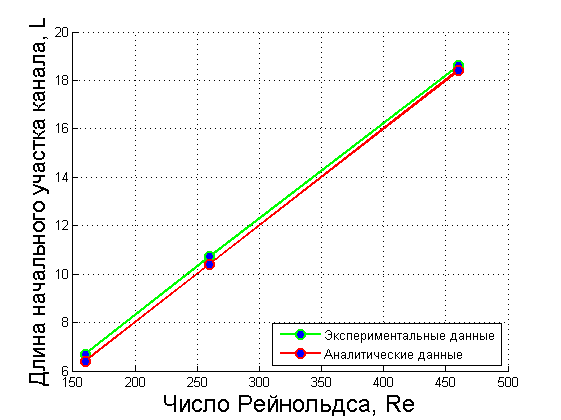
\includegraphics[width = \linewidth]{len}}
    \captionof{figure}{Зависимость $L_{\text{нач.}}$ от $Re$.}
  \end{minipage}
  \hfill
  \begin{minipage}[b]{0.5\linewidth}
  \center{\small Таб. 1: Длина начального участка канала.}\\ \quad \\
    \begin{tabular}[h!]{p{2cm}|>{\raggedleft}p{2cm}>{\raggedleft}p{2cm}}
     $Re$  &   $L_{\text{эксп}}$  &   $L_{\text{ан}}$ \ntb
    \hline
    160  &  6.69  &  6.4 \ntb
    \hline
    260  & 10.72  & 10.4 \ntb
    \hline
    460  & 18.60  & 18.4 \ntb
    \end{tabular}
  \end{minipage}
\end{minipage}

\n
На графике зависимости длины начального участка $L_{\text{нач}}$ от числа Рейнольдса  $Re$ (рис. 11) видно, что зависимость $L_{\text{нач}}$ от $Re$ линейная. 

\subsection{Поле нормального давления}

\noindent $\lambda_{\text{эксп}}$ -- коэффициент сопротивления, полученный из экспериментальных значений по формуле $$\lambda = \frac{2\Delta p}{\Delta L} \cdot \frac{H}{\rho V_{\text{ср}}^{2}}.$$\\
\noindent $\lambda_{\text{ан}}$  -- аналитическая оценка коэффициента сопротивления, полученна при помощи формулы
$$\lambda_{\text{ан}} = \frac{24}{Re}.$$

\begin{center}
   Таб. 3: Коэффициент сопротивления.\\ \quad \\
  \begin{tabular}[h!]{p{2cm}|>{\centering}p{2cm}|>{\centering}p{2cm}|>{\raggedleft}p{2cm}>{\raggedleft}p{2cm}}
  $Re$  &  $\Delta L$  &  $\Delta p$ & $\lambda_{\text{эксп}}$ & $\lambda_{\text{ан}}$ \ntb
  \hline  
  160 & 6.3157 & 0.4718 & 0.1494 & 0.1500  \ntb
  \hline  
  260 & 3.6509 & 0.1692 & 0.0926 & 0.09230 \ntb
  \hline  
  460 & 0.5472 & 0.0148 & 0.0540 & 0.05217 \ntb
  \end{tabular}
\end{center}

\subsection{Коэффициент трения на стенкe канала}

\pic{0.8}{c_down}{Коэффициент трения на стенке канала, $C_f$}

\begin{minipage}{\linewidth}
  \begin{minipage}{0.5\linewidth}
    \center{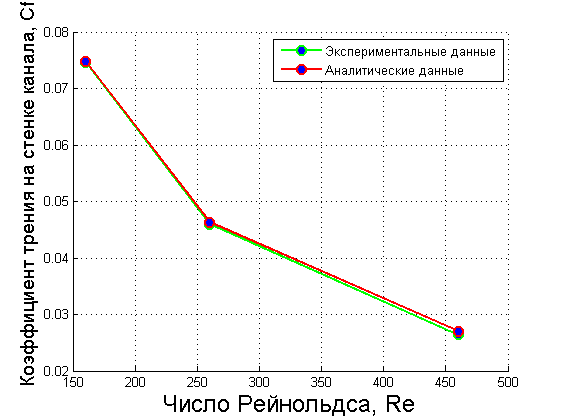
\includegraphics[width = \linewidth]{cf_an}}
    \captionof{figure}{Зависимость $C_f$ от $Re$.}
  \end{minipage}
  \hfill
  \begin{minipage}[b]{0.5\linewidth}
  \center{\small Таб. 3: $C_f$ на стенке канала.}\\ \quad \\
    \begin{tabular}[h!]{p{1.2cm}|>{\raggedleft}p{1.2cm}>{\raggedleft}p{1.2cm}>{\raggedleft}p{1.2cm}}
    $Re$  & $C_f$ & $\lambda$  &  $2C_f$  \ntb
    \hline  
    160 & 0.0746 & 0.1494  & 0.1492 \ntb
    \hline  
    260 & 0.0460 & 0.0926  & 0.0920 \ntb
    \hline  
    460 & 0.0264 & 0.0540  & 0.0528 \ntb
  \end{tabular} 
  \end{minipage}
\end{minipage}

\n
Чем больше $Re$, тем более вязкой жидкость становится, и тем меньшая сила трения на стенках канала наблюдается. 
На рис. 13 видно, что экспериментальный коэффициент трения и полученный по формуле $C_f = \frac{\lambda}{2}$ почти совпадают.

\section{Вывод}

\par Число Рейнольдса характеризует вязкость жидкости, что хорошо показывают эксперименты.
Длина начального участка (п. 2.4) возрастает вместе с $Re$, т.к. течение вязкой жидкости устанавливается тем дольше, чем меньше ее вязкость. 
Коэффициент сопротивления (п. 2.5) убывает с увеличением $Re$, т.к. у менее вязкой жидкости коэффициент споротивления меньше, что подтверждают экспериментальные и аналитические расчеты. То же самое можно сказать и о силе трения на стенке канала (п. 2.6). С развитием течения сила трения устанвливается на определенном значении, тем меньшем, чем больше число Рейнольдса.

\end{document}	
